\documentclass[[12pt]{article}
\usepackage{graphicx}

\title{PROGRAMMING LANGUAGES}
\author{Clement Obieke}

\begin{document}
	\maketitle
	\newpage
	\section* {\Huge{Java}}	
		
\includegraphics[width= 0.1\linewidth]{pics/Jicon.png} \raggedright\\
		\begin{minipage}{0.59\linewidth}		
			\paragraph{}
			\textbf{\large James Gosling designed the Java computer language. James Gosling, Patrick Naughton and Mike Sheridan started the creation of java in June 1991. The name of the team responsible for its development  were called the Green Team.}					
		\end{minipage}
		\begin{minipage}{0.39\linewidth}
			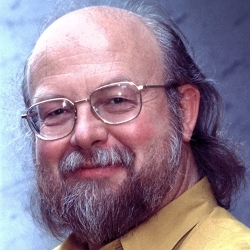
\includegraphics[width= \linewidth]{pics/James.jpg}
		\end{minipage}
	\subsection*{\Large \underline{The creation of Java}}
			\paragraph{}			
			The original design of Java was for television, but it was a bit complex for the digital television at the time. \\
			
			Java’s ability to cater for the multimedia industry showed that it was particularly well suited for the Web. \\
			Java was originally titled as ‘Oak’. The name Java was gotten from an island in Indonesia where the java coffee was produced. Java’s name was changed by James Gosling as he had a cup of coffee by his office.
			
	\subsection*{\underline{Application of Java}}
			\paragraph{}
			Java is used openly to create Consoles, GUI’s, Web Applications, Mobile applications and game development. Some examples of projects created with java are:\\
			\begin{enumerate}
				\item 	NASA world wind
				\item 	Google docs
				\item 	Netflix
				\item 	Spotify 
				\item 	Minecraft etc.
			\end{enumerate}
		
			
	\subsection*{\underline{Java IDE}}
			\paragraph{}
			Java is a programming language that uses a compiler to run its code. Some example of java compilers are:\\
			\begin{enumerate}
				\item Oracle
				\item NetBeans
				\item BlueJ
			\end{enumerate}
			
	\newpage
	\section* {\Huge{Python}}	
				
\includegraphics[width= 0.1\linewidth]{pics/Plogo.png} \raggedright\\
		\begin{minipage}{0.59\linewidth}		
			\paragraph{}
			\large Python was designed by Guido van Rossum. Its main aim was for the purpose of code readability, and its simple syntax allowed programmers to create projects with fewer lines of code.	
		\end{minipage}
		\begin{minipage}{0.39\linewidth}
			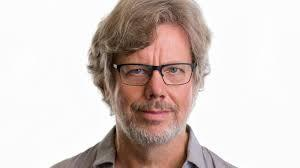
\includegraphics[width= \linewidth]{pics/Pimage.jpg}
		\end{minipage}
		\subsection*{\Large \underline{The creation of Python}}
	\paragraph{}			
		Guido van Rossum started his work on python in the late 1980s in the Netherlands. It was first released in 1991 as python version 0.9.0. When Python was being created, Guido van Rossum got the idea for the name by reading a scripts from “Monty Python's Flying Circus”, this was an early BBC comedy series. This resulted in the language being called Python.\\
		
		The python language is one of the easiest to understand programming languages available because it has a small learning curve and its syntax is simplified, due to its easy usage python codes can be easily written than other programming languages, though it tends to have longer processing time. Either way python is still one of the worlds most popular programming language.
		
	\subsection*{\underline{Application of Python}}
		\paragraph{}
		 Python can be applied in areas of AI and machine learning, Data visualisation, Data analytics, Programming applications, Web development, Language development, Game development and so on.
		 Some  examples of projects created using python are:
		 

		\begin{enumerate}
			\item 	Youtube
			\item 	Instagram
			\item 	Pinterest
	\end{enumerate}
	
	
	
	\subsection*{\underline{Pyhton IDE}}
	\paragraph{}
	(Integrated Development and Learning Environment) IDLE comes default with the installation of the Python language.
	Meaning that IDLE is Python's own IDE.
	\paragraph{}
	Python share a few similarities Java and C++. The both of the languages permit strong cross-platform support and allow for the use of extensive standard libraries. Though python is said to run three times slower than java, python usually takes less lines of code to perform similar tasks.
	
	\newpage
	\section* {\Huge{C\#}}	
	
\includegraphics[width= 0.1\linewidth]{pics/Clogo.png} \raggedright\\
	\begin{minipage}{0.55\linewidth}		
		\subsection*{\Large \underline{The creation of C\#}}
		\paragraph{}			
		\large Anders Hejlsberg created a team to design a new language at the time called Cool. Cool was basically an abbreviations meaning  “C-like Object Oriented Language“. The name "Cool" would have been its name but Microsoft decided the language should be renamed to “C\#”. It changed around the time the .NET project was announced at July 2000.
				
	\end{minipage}
	\begin{minipage}{0.39\linewidth}
		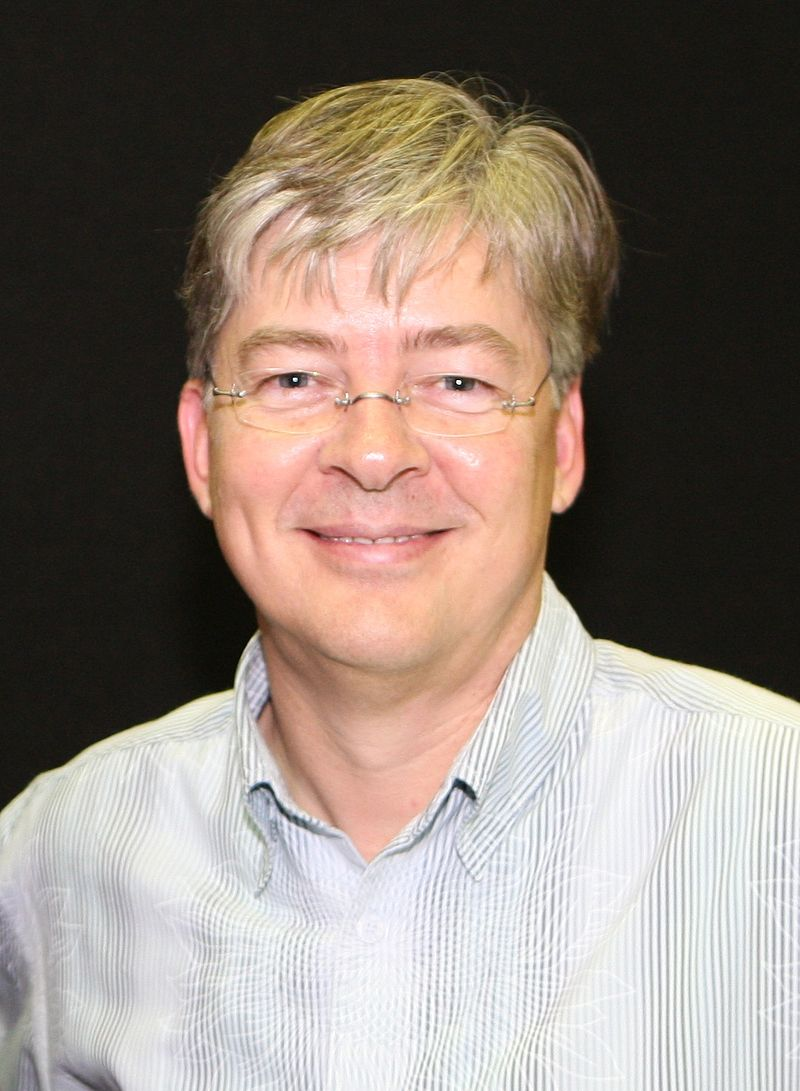
\includegraphics[width= \linewidth]{pics/Anders.jpg}
	\end{minipage}
	
	\subsection*{\underline{Application of C\# }}
	\paragraph{}
	C\# is applied areas like mobile apps, desktop apps, websites, enterprise software, cloud-based services, and games. It has been used to create lots of game.\\
	
	Some projects created with C\# are:

	
	\begin{enumerate}
		\item 	Microsoft Visual Studio
		\item 	Paint.NET
		\item 	Windows Installer XML
		\item 	Unity
			
		
			
	\end{enumerate}
	
	
	\subsection*{\underline{C\# IDE}}
	\paragraph{}
	Some examples of IDEs that support C\# are:

	\begin{enumerate}
		\item	Microsoft visual studio 
		\item	MonoDevelop
		\item	Visual studio code
	\end{enumerate}
	\paragraph{} 
		C\# shares similarities with C++, though it has more features since it is newer.
		
	\newpage
		
	\section* {\Huge{C++}}	
	
\includegraphics[width= 0.1\linewidth]{pics/C+logo.png} \raggedright\\
	\begin{minipage}{0.59\linewidth}		
		\paragraph{}
		\large C++ was developed by Bjarne Stroustrup at Bell Laboratories in 1979. C++ is basically C with object-oriented features plus other minor improvements, previously it was nicknamed as “C with Objects”. Stroustrup called it C++ in 1983.		
	\end{minipage}
	\begin{minipage}{0.39\linewidth}
		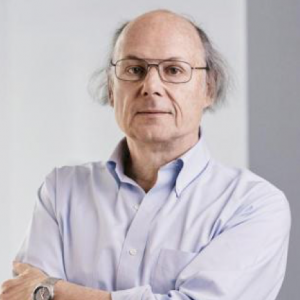
\includegraphics[width= \linewidth]{pics/stroustrup_500.png}
	\end{minipage}
	\subsection*{\Large \underline{The creation of C++ }}
	\paragraph{}
	Bjarne Stroustrup  desired an efficient and versatile language similar to C, one that was also capable of  performing  high-level functions. C++ is the fourth popular programming language. C++ is still popular due to its performance, reliability, and the wide variety of uses.
				
	
	\subsection*{\underline{Application of C++}}
	\paragraph{}
	C++ is applied in areas like Operating systems, Web browsers, Game development, Machine learning tools, AR/VR applications, IoT devices, Databases and Scientific research.
	Some of the projects that use C++ are:
	
	
	\begin{enumerate}
		\item Windows XP
		\item Windows ME
		\item Microsoft Office
		\item Internet Explorer
		\item MySQL
		\item And most of the software from Microsoft is developed using C++ 
		
		
	\end{enumerate}
	
	
	\subsection*{\underline{C++ IDE}}
	\paragraph{}
	Some IDEs that support C++ are:
	
	
	\begin{enumerate}
		\item Eclipse 
		\item Microsoft Visual Studio
		\item CLion
		\item CodeLite
		\item Code::Blocks
	\end{enumerate}

	\newpage
	
	\section* {\Huge{HTML}}	
	
\includegraphics[width= 0.1\linewidth]{pics/html5_logo.png} \raggedright\\
	\begin{minipage}{0.59\linewidth}		
		\paragraph{}
		\large Hypertext Mark-up Language is a computer language deals in the creation of web pages and online applications. HTML was created by Tim Berners-Lee in the year 1993.		
	\end{minipage}
	\begin{minipage}{0.39\linewidth}
		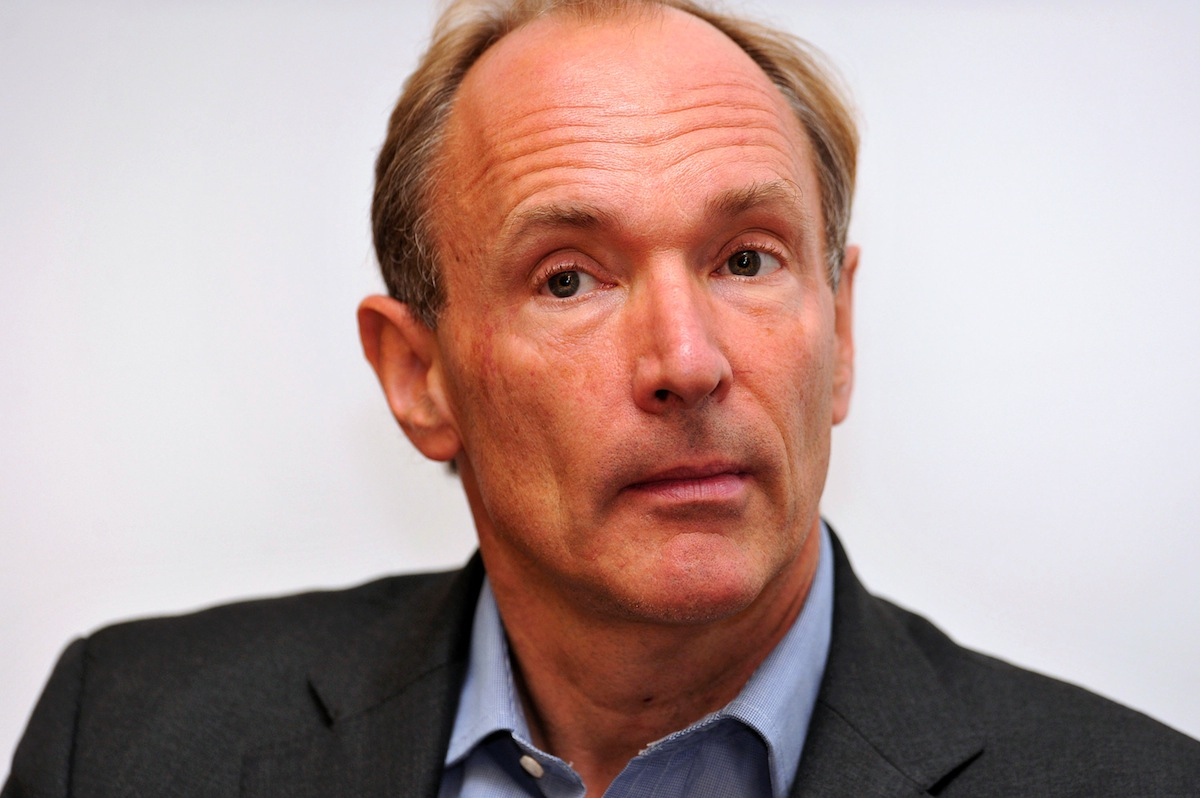
\includegraphics[width= \linewidth]{pics/tbl.jpeg}
	\end{minipage}
	\subsection*{\Large \underline{The creation of HTML}}
	\paragraph{}
	HTML was originally created to allow those who did not understand SGML (a more complex system) to publish
	Scientific documents.\\
	It however became used by those outside the scientific community, Since HTML was simple to learn. As World Wide Web grew, HTML began to quickly spread over and become a common place use.\\
	Nowadays, HTML is used for creating web applications, designing sites and web pages. It is now usually paired with Cascading Style Sheets(CSS) and JavaScript.\\
	\paragraph{}
	HTML is interpreted by web browsers and it is used to create text, images for websites. Items of the Hyper text mark-up language are defined in the browser, and these are customised though the use of CSS.\\	
	HTML helped in the exchange of data by creating the ability to link documents together by the use of hyperlinks. This is how the name HyperText Mark-up language was chosen.	
	\subsection*{\underline{Application of HTML}}
	\paragraph{}
	The application of HTML revolves around the use of the internet. It is majorly use for Web pages development, Maintenance and management.\\
	
	\subsection*{\underline{HTML IDE}}
	\paragraph{}
		Some examples of IDEs that allow the use of HTML are:
	\begin{enumerate}
			\item 	UltraEdit.
		\item 	NoteTab.
		\item 	Notepad++
		\item 	Sublime Text.
		\item 	Komodo IDE.
		\item 	Visual Studio Code
		
	\end{enumerate}

	\newpage
\end{document}